\documentclass{standalone}

\usepackage{amssymb}
\usepackage{amsthm}
\usepackage{amsmath}


\usepackage{tikz}
\usetikzlibrary{shapes,backgrounds,calc,patterns}


\begin{document}
	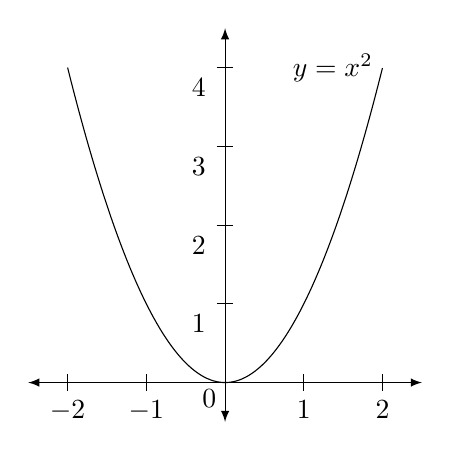
\begin{tikzpicture}
	\draw[latex-] (-2.5,0) -- (0,0) ;
	\draw[-latex] (0,0) -- (2.5,0) ;
	\draw[latex-] (0,-.5) -- (0,0);
	\draw[-latex] (0,0) -- (0,4.5);
	\foreach \x in  {-2,-1,1,2}
	\draw[shift={(\x,0)},color=black] (0pt,3pt) -- (0pt,-3pt);
	\foreach \x in {-2,-1,1,2}
	\draw[shift={(\x,0)},color=black] (0pt,0pt) -- (0pt,-3pt) node[below] 
	{\(\x\)};
	\foreach \x in  {1,2,3,4}
	\draw[shift={(0,\x)},color=black] (-3pt,0pt) -- (3pt,0pt);
	\foreach \x in  {1,2,3,4}
	\draw[shift={(0,\x)},color=black] (0pt,0pt) -- (-3pt,0pt) node[below left=.5pt] 
	{\(\x\)};
	\node at (-.2,-.2) {\(0\)};
	\draw[smooth,samples=100,domain=-2:2,variable=\x] plot ({\x},{\x*\x}) node[left] {\(y=x^2\)};
	\end{tikzpicture}
\end{document}